../cictikz/src/cictikz/data/tex/cictikz_preamble.tex

% Band diagram through gate, oxide and bulk of a fictive MOSFET with no
% applied voltage: one shared Fermi level, p-type bulk.

\definecolor{lblred}{RGB}{160,25,35}
\definecolor{eblue}{RGB}{85,155,235}

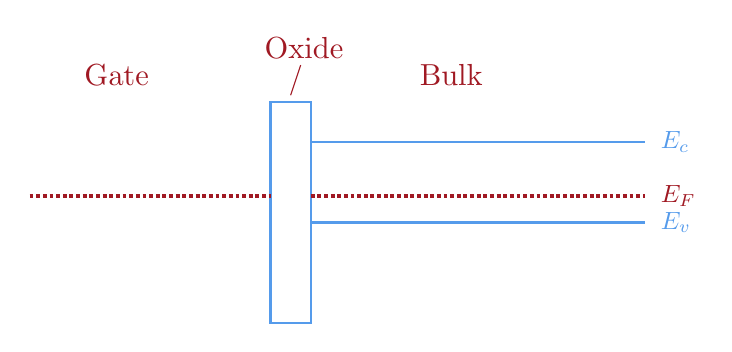
\begin{tikzpicture}[scale=0.85]

  % oxide
  \draw[eblue, thick] (3.9,-0.4) rectangle (4.5,2.9);

  % gate: metallic, Fermi level at the conduction band edge
  \draw[lblred, densely dotted, line width=1.4pt] (0.3,1.5) -- (3.9,1.5);

  % bulk: p-type, E_F closer to the valence band
  \draw[eblue, thick] (4.5,2.3) -- (9.5,2.3);
  \node[eblue, anchor=west, scale=0.9] at (9.6,2.3) {$E_c$};
  \draw[lblred, densely dotted, line width=1.4pt] (4.5,1.5) -- (9.5,1.5);
  \node[lblred, anchor=west, scale=0.9] at (9.6,1.5) {$E_F$};
  \draw[eblue, thick] (4.5,1.1) -- (9.5,1.1);
  \node[eblue, anchor=west, scale=0.9] at (9.6,1.1) {$E_v$};

  % region labels
  \node[lblred, anchor=center, scale=1.1] at (1.6,3.3) {Gate};
  \node[lblred, anchor=center, scale=1.1] at (4.4,3.7) {Oxide};
  \draw[lblred, thin] (4.35,3.45) -- (4.2,3.0);
  \node[lblred, anchor=center, scale=1.1] at (6.6,3.3) {Bulk};

\end{tikzpicture}
\end{document}
